\documentclass[11pt, a4paper]{article}

\usepackage{amsmath}
\usepackage{amsfonts}
\usepackage{graphicx}
\usepackage[export]{adjustbox}
\usepackage{hyperref}
\usepackage{fullpage}
\usepackage{caption}
\usepackage{listings}
\usepackage[dvipsnames]{xcolor}
\usepackage{gensymb}
\usepackage{wrapfig}
\hypersetup{
    bookmarks=true,         % show bookmarks bar?
    unicode=false,          % non-Latin characters in Acrobat’s bookmarks
    pdftoolbar=true,        % show Acrobat’s toolbar?
    pdfmenubar=true,        % show Acrobat’s menu?
    pdffitwindow=false,     % window fit to page when opened
    pdfstartview={FitH},    % fits the width of the page to the window
    pdftitle={My title},    % title
    pdfauthor={Author},     % author
    pdfsubject={Subject},   % subject of the document
    pdfcreator={Creator},   % creator of the document
    pdfproducer={Producer}, % producer of the document
    pdfkeywords={keyword1, key2, key3}, % list of keywords
    pdfnewwindow=true,      % links in new PDF window
    colorlinks=true,       % false: boxed links; true: colored links
    linkcolor=Blue,          % color of internal links (change box color with linkbordercolor)
    citecolor=green,        % color of links to bibliography
    filecolor=magenta,      % color of file links
    urlcolor=red           % color of external links
}

\title{MAAS - Project Report \\Commitment Issues}
\author{Sushant Vijay Chavan\\Ahmed Faisal Abdelrahman\\Abanoub Abdelmalak}
\date{\today}

\begin{document}
\maketitle
\newpage
\tableofcontents{}
\newpage

\section{Introduction}
\paragraph{}
In this project, we implemented two stages and a visualization component of the Flying Saucers Bakery, an inter-group cooperative project for the Multi-Agent and Agent Systems course. The stages this group was responsible for were the final two: packaging and delivery. Initially, the group was tasked with formulating an architecture for the entire project, including specifying the agents, their communication mechanisms, and the flow of a bakery's processes. Subsequently, the group assumed responsibility for the afore-mentioned stages, implementing them end-to-end, and working to integrate them with the agents developed by other teams.

\paragraph{}
As per the specifications of the project, the packaging stage was developed so as to receive baked bakery products, perform certain post-baking steps, and packaging them into separate boxes to be passed on to the next stage. The delivery stage was designed to receive these, aggregate them based on customer orders, and facilitate delivering them to the right customers most efficiently. This involved distributing them among trucks, which travel around the street network to deliver orders from bakeries to customers. A graph visualizer application of the street network was developed to enable visualization of this stage.

\paragraph{}
All agents were defined in each stage to be responsible for a certain task, and the design decisions were agreed upon among the group members. Each member was then responsible for developing certain agents, while adhering to the defined architecture and agent communication constraints. In addition, certain data structures were encapsulated in objects. These were needed for certain functionalities, but did not justify implementation as agents, since no communication or decision-making was made on their part.

\paragraph{}
Throughout the project, developed agents had to be appropriately maintained and updated to keep up with changes to the upstream repository of the project. This was particularly necessary for the interface agents (loading bay and mailbox agents), since they were standardized and used by multiple groups. During the project git issues, pull requests, reviews, and other tools were utilized to enable seamless integration with the other groups.

\paragraph{}
This report is structured as follows. Section 2 and 3 elaborate on the packaging and delivery stages, respectively, including descriptions of the architectures, the developed agents, and message specifications for the interface agents. Section 3.2 explains the graph visualization of the delivery phase's street network. Finally, section 4 contains instructions for running both stages, and running separate stages on separate machines.

\section{Packaging Stage}\label{PackagingStage}
\paragraph{}
This stage deals with completion of the post baking stages and then packaging the products into boxes so that they are ready for delivery. The stage receives the baked and cooled products from the cooling racks and preforms the final preparation of the products such as sprinkling and decorating according to the recipe for the product. Once the products are ready, they are packed into boxes based on the delivery date priority of the orders. Once all the boxes of a given product type in an order are ready, they are sent to the delivery stage for transportation.

\paragraph{}
Figure \ref{PackagingArchitecture} gives an overview of the architecture of the packaging stage. This stage consists of three agents and in addition communicates with the CoolingRacks agent to receive the cooled products. The GenericItemProcessor takes care of all the post-baking steps, where as the packaging agent boxes the products based on the order priority. The Loading bay keeps track of the produced quantity of the products and informs the delivery stage whenever all products of a type in an order are ready.

\begin{figure}[h!]
	\centering
	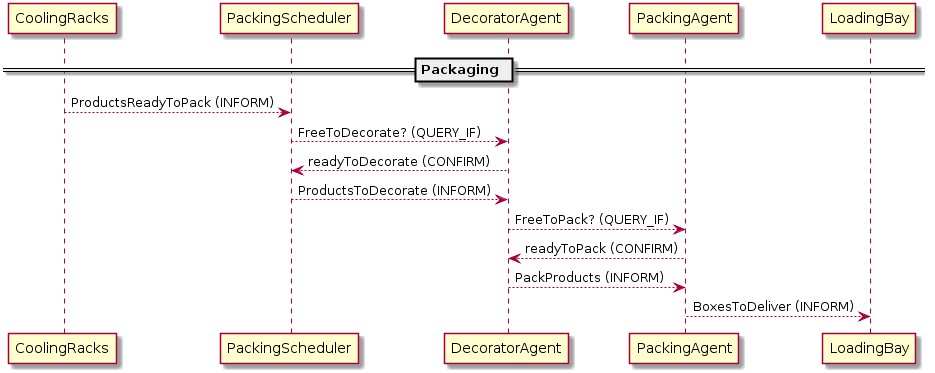
\includegraphics[width=\textwidth]{../Architecture/Architecture_Packaging.png}
	\caption{Packaging Stage Architecture}
	\label{PackagingArchitecture}
\end{figure}

\paragraph{}
The output of this stage is a set of boxes that consists of a fulfilled item from a customer order. For example, if a customer order consists of 10 breads and 15 donuts, assuming that the loading bay sees that the 15 donuts of this order are available, it sends these boxes to the delivery stage. Please note that not all products of this order are yet complete and that the loading bay will wait until all the breads of this order are available before sending out a new message to the delivery stage.

\hfill\break
\subsection{Agents}\label{PackagingAgents}
\subsubsection{Entry Agent (Developer: Sushant)}
\paragraph{}
In order to test the two developed stages independently of the other stages, we need an agent that can trigger the cooling racks agent to start the simulation. The EntryAgent fulfills this requirement. Using this agent, it is possible to simulate that the products from of an order have been baked and are ready for cooling, which then starts the two following stages until the order has been delivered to the customer. It should be noted that the EntryAgent simply uses the order information available in the scenario files and does not generate any data on its own.

\paragraph{}
The Entry agent has two functionalities. First, it reads the order details from the currently active scenario directory and then generates dummy messages that inform the cooling rack that the products of an order are ready. These messages are then sent to the cooling rack at the delivery time mentioned in the scenario file. Therefore, the first part of this agent acts as the trigger for the two stages. Since the order processor agent was also not available on the upstream repository, we added the order processor functionality as the second functionality of the entry agent. Whenever an order is sent to the cooling rack, a corresponding order information is also broadcast to all agents. We used the same  message format as the actual order processor. In this way we ensure that all our agents are compatible with the actual order processor, whenever it is available.

\subsubsection{Generic Item Processor (Developer: Abanoub)}
This agent is responsible for receiving the items sent by the cooling racks, prepare them for packaging and send them to the packaging agent to be packed. Based on the scenario files used for the simulation and the bakery this agent belongs to, it creates a list with all the products. Using the scenario file, each product is acquired with the processes it needs to be ready for packaging and their duration. After preparing this list of the products with their features, the agent starts to receive products from the cooling racks and start executing the processes one by one for each of them until it is done. The products are sent to the packaging agent as soon as they are processed and all the time needed for each of the processes is finished.
\subsubsection{Packaging Agent (Developer: Sushant)}
\paragraph{}
This agent is responsible for receiving the ready products and then packaging them into boxes. The packaged boxes are then sent to the loading bay so that they can be dispatched to the customer. This agent prioritizes the packaging of the received products based on the delivery time of the orders. 
\paragraph{}
For example, assume we have two orders requiring 10 and 20 breads respectively and that the delivery date of the first order is earlier than that of the second. Now if we receive 20 breads from the previous stage, the packaging agents first boxes the 10 breads for the first order and sends them to the loading bay. It then packages the remaining 10 breads as a part of the second order. It must be noted that the packaging agent sends out the boxes as soon as they are full. It expects the loading bay to store the boxes until all boxes of a product type in an order are ready.

\subsubsection{Loading Bay Agent (Developer: Ahmed)}
\paragraph{}
The loading bay agent acts as the interface between the packaging stage and the delivery stage. Aside from transferring boxes of packaged products along from the packaging agent to the order aggregator agent, it is responsible for sending boxes of products only when all of the products of a certain type, in a respective order have been fulfilled.
\paragraph{}
The agent receives two types of messages, one from the preceding packaging agent and another from the common order processing agent. The former sends a list of boxes of products that belong to an order, while the latter provides the list of products needed to fulfill every order, among the other order details. The agent receives boxes of products and retains them with their order IDs. Meanwhile, it maintains all orders' details and continuously checks if it has all the products of a certain type needed for any order. Once an order's products of a particular type are all present, it dispatches a message to the next agent containing a list of all the boxes containing these products.
	
\pagebreak
\hfill\break
\textbf{Message Descriptions}:

\hfill\break
\textbf{(Incoming) Packaged Boxes Message:}

\hfill\break
\textbf{Description}:	
The LoadingBayAgent receives boxes of packaged products from a packaging agent in a message of the following format:
\hfill\break
\textbf{Performative}: INFORM
\hfill\break
\textbf{Sender}: AID of the packaging agent
\hfill\break
\textbf{Receiver}: AID of the LoadingBayAgent
\hfill\break	
\textbf{Conversation ID}: "boxes-ready"

\hfill\break
Figure \ref{loadingbaymsg1example} shows an example of the contents of the message.
\begin{figure}[h!]
	\centering
	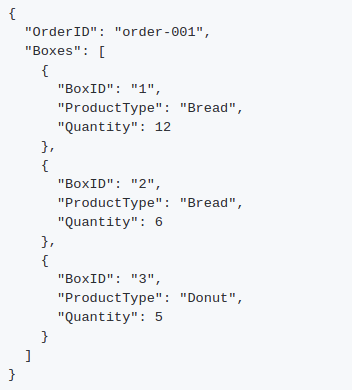
\includegraphics[width=0.4\textwidth]{../images/loadingbaymsg1example.png}
	\caption{Packaged Boxes Example Message}
	\label{loadingbaymsg1example}
\end{figure}

\hfill\break
\textbf{(Outgoing) Fulfilled Order Boxes Message}:
	
\hfill\break
\textbf{Description}:
The LoadingBayAgent agent sends the order aggregator agent a message containing the details of boxes of products belonging to a particular order. It does so once it receives boxes that contain all of the products of a type that fulfill that order. The message is of the following format:
\hfill\break
\textbf{Performative}: INFORM
\hfill\break
\textbf{Sender}: AID of the LoadingBayAgent
\hfill\break
\textbf{Receiver}: AID of an OrderAggregatorAgent

\hfill\break	
The message is of the same format as the incoming message, and an example can be seen on Figure \ref{loadingbaymsg1example}.

\newpage
\section{Delivery Stage}\label{DeliveryStage}
\paragraph{}
This stage handles the delivery of the packaged boxes from the bakery to the customers. The inputs to this stage are a set of boxes from the packaging stage as described in the section \ref{PackagingStage}. This stage waits until all the products of an order are ready for dispatch and then requests the trucks for transportation of these boxes. Once the orders have been delivered to the customer, the trucks post the status of the delivery to the mailbox, which then informs the concerned customer agent.

\paragraph{}
This stage consists of five agents as shown in the architecture diagram in figure \ref{DeliveryArchitecture}. In addition, this stage talks with two other agents: \textit{LoadingBayAgent} and the \textit{GraphVisualizationAgent}. The figure gives an overview of the communication happening between the agents in order to deliver an order received from the LoadingBayAgent. The visualization of the delivery stage will be explained in detail in section \ref{GraphVisualizationAgent}. However, it is helpful to know that the only agents that need to communicate with the GraphVisualizationAgent are the StreetNetworkAgent and the TruckAgents. 

\begin{figure}[h!]
	\centering
	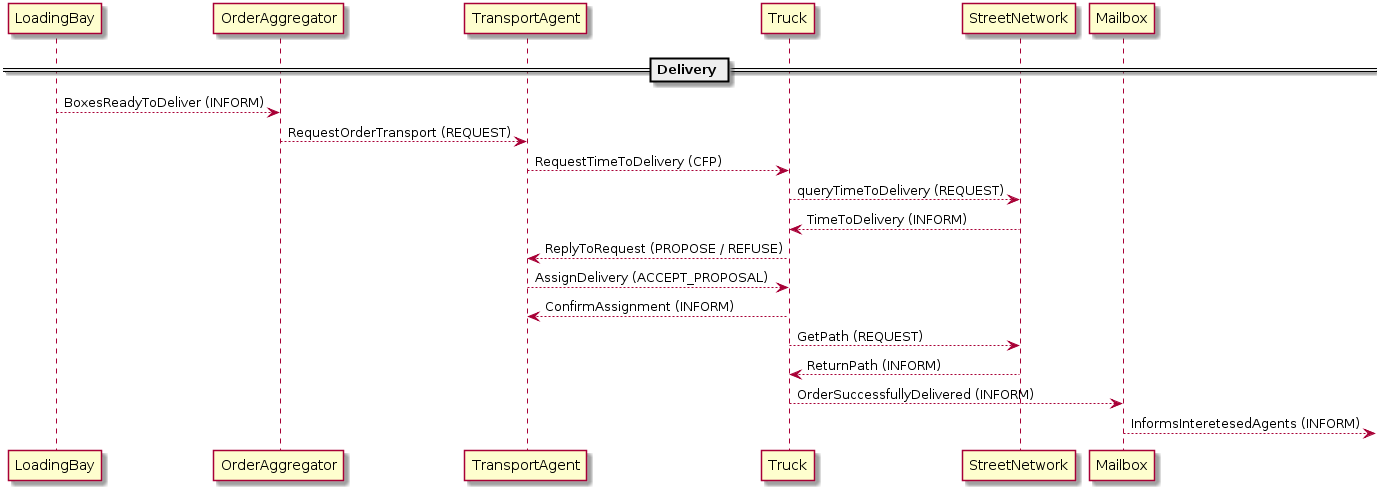
\includegraphics[width=\textwidth]{../Architecture/Architecture_Delivery.png}
	\caption{Delivery Stage Architecture}
	\label{DeliveryArchitecture}
\end{figure}

\paragraph{}
In order to find the best truck that can deliver the orders, the transport agent of the bakery requests for proposals from the trucks to deliver the order. Each truck which is capable of delivering this order then queries the StreetNetwork to find the time needed to complete its current task, return to the bakery to collect the products, and then move towards the customer. These estimates are then sent back to the transport agent, which then chooses the truck that has the least time to delivery.  Section \ref{DeliveryAgents} provides a detailed description of all the agents that are a part of the delivery stage.

\subsection{Agents}\label{DeliveryAgents}
\subsubsection{Order Aggregator (Developer: Abanoub)}
Based on the idea that the loading bay will send the boxes of products that are complete, this agent is responsible for gathering all the needed information about the boxes sent by the loading bay and forward the complete orders to the transport agent after it makes sure that the order is fulfilled. The agent works as follows: it keeps track of all the orders that the order processor broadcast. Then it waits until the loading bay sends boxes to be delivered. The boxes with their order id are used to check the order fulfillment and then send the full order to the transport agent.

\subsubsection{Transport Agent (Developer: Abanoub)}
This agent is responsible for receiving the boxes of fulfilled orders from the order aggregator, getting the location of the bakeries and the customers of this specific order, assigning the order to the trucks with the best delivery time and handing the orders to the trucks when they arrive at the bakeries. This is achieved as follows: It keeps updating a list of customers IDs associated with their orders IDs sent by the order processor. Then the cycle starts when it receives boxes from the order aggregator. It uses the details sent by the order aggregator to find the location of the customer and the bakery associated with this order. After that it communicates with all the trucks to call for proposals with the time each of them needs to deliver the order, then chooses the truck with the best time and assigns the order to it. When the truck arrives at the bakery to pick the order it gives the boxes to it.\\
Each transport agent is associated with a bakery.
\subsubsection{Truck Agent (Developer: Sushant)}
This agent is responsible for collecting orders from a bakery and delivering them to the customers. Each truck is associated with a transport company and multiple transport companies could exist. It is responsible for querying the estimated delivery time for an order and proposing this to the transport agent. If the proposal is accepted, it is also responsible for moving towards the bakery to collect the orders and then moving towards the customers to deliver them. Finally, it also informs the status of the delivery (such as the time of delivery, number of boxes) to the mailbox. Due to its highly dynamic nature, this agent has an extensive communication with other agents, as can be seen from the figure \ref{DeliveryArchitecture}. It must be noted that with the current implementation, every truck can accept at most one extra order in addition to the one it is currently handling. 
	
Additionally this agent also communicates with the GraphVisualizationAgent in order to send its position and status updates for visualization. 
\subsubsection{Street Network Agent (Developer: Ahmed)}
\paragraph{}
The street network agent is responsible for maintaining the world `map' in a graphical representation, containing the locations of all places, connections between them, and the distances, as specified in each scenario. Additionally, it provides navigational and temporal information to truck agents. This includes the paths that they must traverse to get from one location to another, and the time it would take to do so.
\paragraph{}
With the help of a few helper classes, such as \textit{Graph}, \textit{Vertex}, and \textit{Edge}, the agent stores and updates (if necessary) the map as a directed graph. It makes use of an implementation of the Dijkstra algorithm that facilitates a graph search to find the shortest path between two nodes. This implementation is adapted from Lars Vogel's, which can be found \href{http://www.vogella.com/tutorials/JavaAlgorithmsDijkstra/article.html}{in this link}.
\paragraph{}
The agent communicates with truck agents and the graph visualization agent. The graph visualization agent constructs the visualization of the street network by obtaining the graph representation of the map from the street network agent.
\subsubsection{Mailbox Agent (Developer: Ahmed)}
\paragraph{}
The mail box agent is the interface agent between the final delivery stage and the customers. It receives the details of delivered orders from truck agents, and confirms these deliveries to the concerned customer agents. It can be extended to relay this information to any agent who requires it.
\paragraph{}
The agent sends a message which contains all the relevant details of a confirmed delivery, such as the truck (and delivery company) that delivered it, the customer, the time, and the contents of the delivery.

\hfill\break
\textbf{Message Descriptions}:

	\begin{wrapfigure}[]{r}{0.4\textwidth}
		\begin{center}
			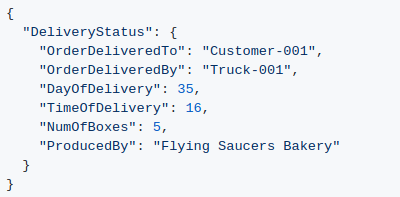
\includegraphics[width=0.4\textwidth]{../images/mailboxmsgexample.png}
		\end{center}
		\caption{Mailbox Example Message}
		\label{mailboxmsgexample}
	\end{wrapfigure}
\hfill\break
\textbf{(Incoming) Truck Message:}

\hfill\break
\textbf{Description}:
The TruckAgent informs the mailbox about a delivered order using the following message:
\hfill\break
\textbf{Performative}: INFORM
\hfill\break
\textbf{Sender}: AID of the TruckAgent that sends this message
\hfill\break
\textbf{Receiver}: AID of the MailboxAgent
\hfill\break
\textbf{PostTimeStamp}: Current system time
\hfill\break
\textbf{Conversation ID}: \textit{orderID}

\hfill\break
Figure \ref{mailboxmsgexample} shows an example of the contents of the message

\hfill\break	
\textbf{(Outgoing) Fulfilled Order Boxes Message:}

\hfill\break
\textbf{Description}:
The mail box relays the delivery status message to the concerned customer and other agents who are interested in knowing the delivery status of the order using the following message:
\hfill\break
\textbf{Performative}: INFORM
\hfill\break
\textbf{Sender}: AID of the MailboxAgent
\hfill\break
\textbf{Receiver}: AID of the Concerned CutomerAgent. If more agents are interested in receiving this message, their AID's will also be added to the receiver list.
\hfill\break
\textbf{PostTimeStamp}: Current system time
\hfill\break
\textbf{Conversation ID}: \textit{orderID}

\hfill\break
The message is of the same format as the incoming message, and an example can be seen on Figure \ref{mailboxmsgexample}.

%	\begin{figure}[h!]
%		\centering
%		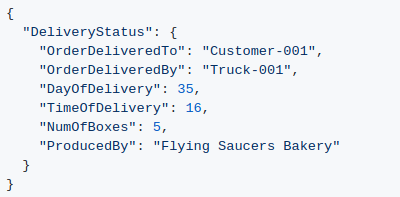
\includegraphics[width=0.5\textwidth]{../images/mailboxmsgexample.png}
%		\caption{Mailbox Example Message}
%		\label{mailboxmsgexample}
%	\end{figure}
	
\pagebreak
	
\subsection{Objects}\label{DeliveryObjects}
The \textit{Graph}, \textit{Vertex}, \textit{Edge}, and \textit{DijkstraAlgorithm} classes are taken from Lars Vogel's implementation of the Dijkstra algorithm. A link to the source code and an accompanying blog post can be found \href{http://www.vogella.com/tutorials/JavaAlgorithmsDijkstra/article.html}{here}.
\subsubsection{Graph}
\paragraph{}
The Graph object implements a directed graph of nodes and edges to be used in the Dijkstra algorithm. It maintains two lists: one consisting of \textit{Vertex} objects, and another of \textit{Edge} objects.

\subsubsection{Vertex}
\paragraph{}
The Vertex object represents a vertex in a directed graph to be used in the Dijkstra algorithm. The class maintains a vertex's, or node's, ID and name as strings, and a few helper functions. For example, an equality helper function that checks whether two vertex objects are equivalent.

\subsubsection{Edge}
\paragraph{}
The Edge object represents an edge in a directed graph to be used in the Dijkstra algorithm. Each edge stores a source vertex/node, a destination node, a unique ID, and a weight value. 

\subsubsection{DijkstraAlgorithm}
\paragraph{}
The DijsktraAlgorithm class implements the Dijkstra algorithm for finding the shortest path between two nodes in a directed graph. This is used in the street network agent to enable returning of paths between two locations, as well as the time needed for the journey, to truck agents which as for this information.


\subsubsection{Box}
\paragraph{}
The box class characterizes the requirements of a box object that has been described in the project description. This class holds a fixed amount of products of a single product type. Box objects can be uniquely identified using the box id. This class also provides helper functions such as adding products to a box, querying its ID and printing the details of the box.
\subsubsection{Order}
\paragraph{}
The order class was implemented to help organize the work with the delivery stage to be used within the transport agent and the order aggregator. This class contains the necessary data to define an order like: order id, customer id, bakery id. Some other features like changing the location of the bakery and the location of the customer associated with each of the orders.
\newpage
\subsection{Graph Visualization Agent (Developer: All)}\label{GraphVisualizationAgent}
\paragraph{}
The graph visualization agent facilitates observing the delivery process of the orders in a graphical way. This agent is capable of displaying the entire street network (consisting of its nodes and edges) and all the trucks present at any given time as shown in figure \ref{VisualizationScreenshot}. JavaFX was used to generate the nice display and we used and modified the implementation of \href{https://stackoverflow.com/a/30696075}{Roland} to generate the graph representation.

\begin{figure}[h!]
	\centering
	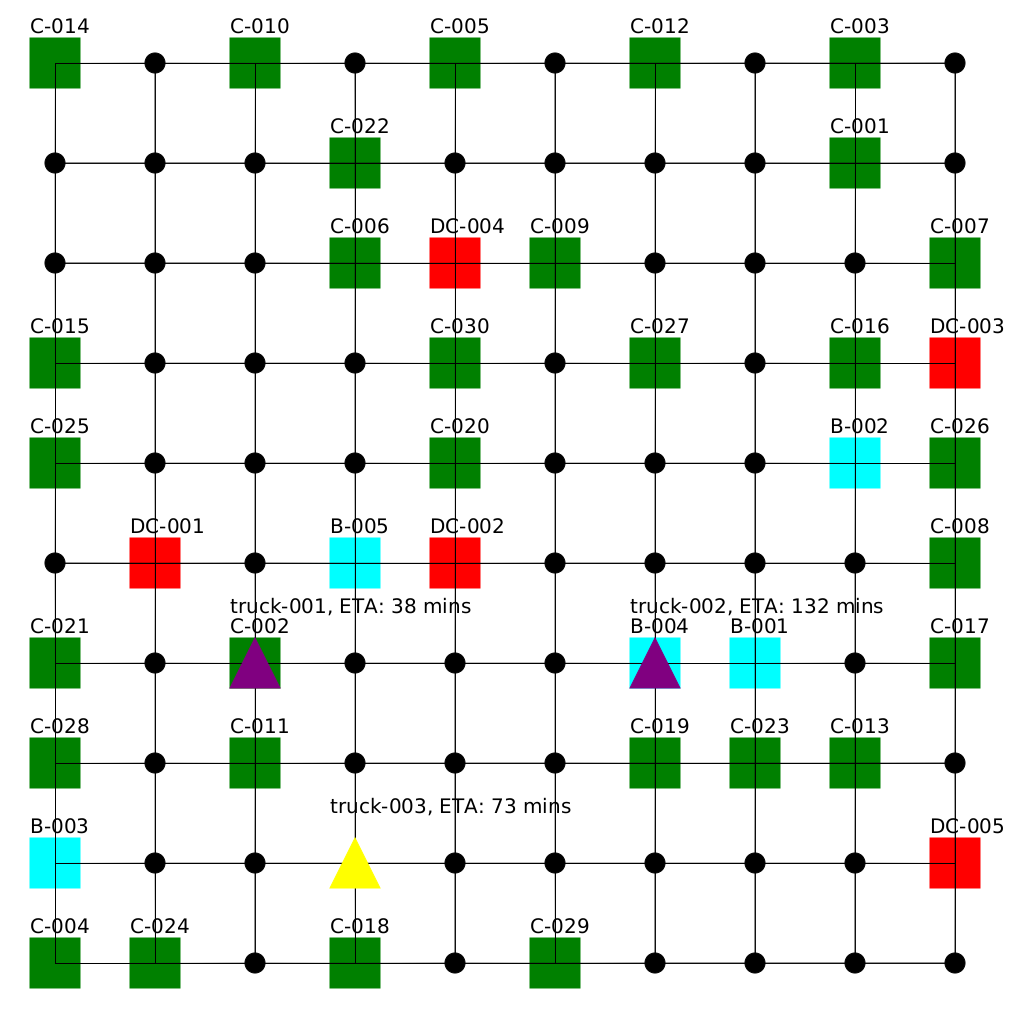
\includegraphics[width=\textwidth]{Visualization.png}
	\caption{Screenshot of Delivery Stage Visualization}
	\label{VisualizationScreenshot}
\end{figure}

\paragraph{}
The nodes of the graph are displayed as either squares (for important nodes such as bakery or customer locations) or small circles. The nodes are then connected by the edges. The squares are further color coded in order to distinguish the type of node. Green represents customers, red delivery companies and cyan bakery locations. The trucks are represented using triangles on the graph and it is possible to update their location based on their actual position in the graph at any time step. Similar to the nodes, the trucks are also color coded to identify their states. Gray represents idle state, yellow moving towards bakery for collecting boxes and purple delivering boxes to a customer. Additionally, the trucks also display the expected time of arrival along their current route.

\paragraph{}
This agent communicates with two agents in the delivery stage. The street network agent sends the street network information (consisting of the nodes and the edges) at startup to the graph visualization agent. Similarly, the trucks inform the graph visualization agent about their start positions. Whenever the position of a truck is updated, a new message is sent to the graph visualization agent informing it about the new position, expected time of arrival and state of the truck.

\section{Usage Instructions}

\subsection{Running the two stages}
In order to run the simulation of these two stages, follow the below steps:
\begin{enumerate}
	\item Clone the repository from \href{https://github.com/HBRS-MAAS/ws18-project-commitment_issues}{GitHub}
	\item Install the gradle version mentioned in the README of the cloned repository.
	\item Ensure that the EntryAgent is active by checking the file \textit{PackagingStageInitializer.java} by uncommenting the below line if it is commented.
	\begin{verbatim}	 \textit{agents.add("EntryAgent:org.commitment_issues.packaging_agents.
	 EntryAgent(" + scenarioDirectory + ")"); \end{verbatim} 
	\item Start the program using the command
	\begin{verbatim}
	gradle run --args='-packaging -delivery -visualization'
	\end{verbatim}
	\item If you get an error saying gradle does not support '\textit{args}'. Then use the below command instead to start the program
	\begin{verbatim}
	./gradlew run --args='-packaging -delivery -visualization'
	\end{verbatim}
\end{enumerate}

\subsection{Running on distributed systems}
Follow these steps to run multiple stages on different systems.
\begin{enumerate}
	\item Connect all systems to the same network.
	\item Search for open ports using the command:
\begin{verbatim}
netstat -lntu
\end{verbatim}
	\item Look for a port whose state is not LISTEN (this will be the PORT used below).
	\item Find the host's IP address using the command: (in field wlp8s0, Inet addr: ...)
\begin{verbatim}
ifconfig
\end{verbatim}
	\item Start the host using the command:
\begin{verbatim}
gradle run --args='-isHost [host ip address] -localPort [PORT] -[STAGE] -noTK'
\end{verbatim}
Example:
\begin{verbatim}
gradle run --args='-isHost 192.168.43.113 -localPort 5353 -packaging -noTK'
\end{verbatim}

	\item Start a client using the command:
\begin{verbatim}
gradle run --args='-host [HOST IP ADDRESS] -port [HOST LISTENING PORT] -[STAGE]'
\end{verbatim}
Example:
\begin{verbatim}
gradle run --args='-host 192.168.43.113 -port 5353 -packaging'
\end{verbatim}
\end{enumerate}

\end{document}\grid
